\documentclass{standalone}
\usepackage{tikz, tikz-cd}
\usetikzlibrary{shapes, decorations.markings}
\begin{document}

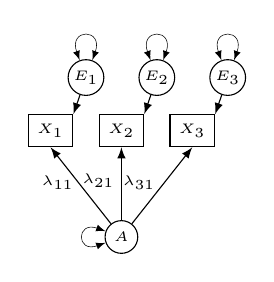
\begin{tikzpicture}[scale=0.9]
\node[draw, circle, inner sep=2] (l1) at (2,2) {\tiny{$A$}};
\node[draw] (o1) at (1,3.5) {\tiny{$X_1$}};
\node[draw] (o2) at (2,3.5) {\tiny{$X_2$}};
\node[draw] (o3) at (3,3.5) {\tiny{$X_3$}};
\node[draw, circle, inner sep=1] (l2) at (1.5,4.25) {\tiny{$E_1$}};
\node[draw, circle, inner sep=1] (l3) at (2.5,4.25) {\tiny{$E_2$}};
\node[draw, circle, inner sep=1] (l4) at (3.5,4.25) {\tiny{$E_3$}};
% Arrows
\draw [->, thin, >=latex] (l1)--(o1.south) node [midway, left, xshift=1, yshift=1] {\tiny{$\lambda_{11}$}};
\draw [->, thin, >=latex] (l1)--(o2.south) node [midway, left, xshift=1, yshift=1] {\tiny{$\lambda_{21}$}};
\draw [->, thin, >=latex] (l1)--(o3.south) node [midway, left, xshift=1, yshift=1] {\tiny{$\lambda_{31}$}};
\draw [->, thin, >=latex] (l2)--(o1.north east);
\draw [->, thin, >=latex] (l3)--(o2.north east);
\draw [->, thin, >=latex] (l4)--(o3.north east);
% Residuals:
\draw[<->, very thin, >=latex] (l2) to [out=70,in=110,looseness=7] (l2);
\draw[<->, very thin, >=latex] (l3) to [out=70,in=110,looseness=7] (l3);
\draw[<->, very thin, >=latex] (l4) to [out=70,in=110,looseness=7] (l4);
\draw[<->, very thin, >=latex] (l1) to [out=160,in=200,looseness=7] (l1);
\end{tikzpicture}

\end{document}